\begin{figure}[h!]
    \centering
	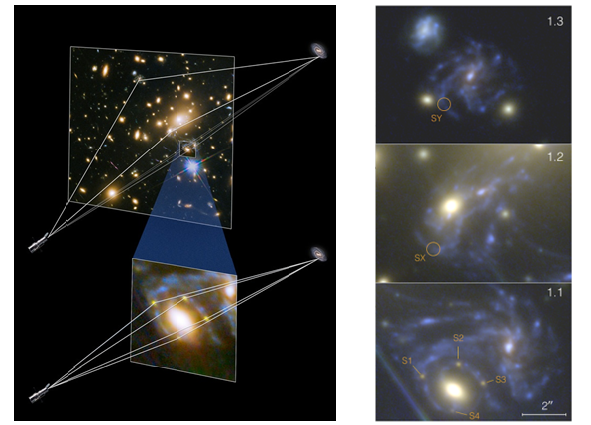
\includegraphics[scale=0.8]{pics/snrefsdal.png}
	\caption{Слева: схематичное изображение хода лучей от SN Refsdal к  наблюдателю (источник: Space Telescope Science Institute). Справа: изображения SN Refsdal (\cite{treu2015}) \label{fig:snrefsdalfig}}
\end{figure}

SN Refsdal находится в рукаве спиральной галактики на красном смещении $z_S= 1.49$, которая линзируется скоплением галактик MACSJ1149.6+2223, находящимся на $z_L= 0.54$, таким образом, что существуют сразу три изображения родительской спиральной галактики (изображения 1.1, 1.2 и 1.3 на правой панели Рисунка \ref{fig:snrefsdalfig}). При этом в изображении 1.1 сверхновая дополнительно линзируется эллиптической галактикой скопления таким образом, что формируются четыре её изображения S1-S4 (правая нижняя панель Рисунка \ref{fig:snrefsdalfig}), расположенных в виде “креста Эйнштейна”. Изображение сверхновой SX (средняя панель справа) интересно тем, что его появление в 2015 году было предсказано с высокой точностью (\cite{kelly2014},\cite{treu2015}). Согласно теоретическим оценкам, SY (правая верхняя панель) - это изображение сверхновой, которое “вспыхнуло” ~20 лет назад (\cite{kelly2014}) и уже угасло.
